\documentclass[11pt]{article}
\usepackage{amsmath}
\usepackage{graphicx}
\usepackage{booktabs}
\usepackage{geometry}
\usepackage{float}
\usepackage{hyperref}

\geometry{margin=1in}

\title{Homework 4: Principal Component Regression (PCR)}
\author{Your Name}
\date{\today}

\begin{document}

\maketitle

\section{Introduction}
This report presents an analysis of Principal Component Regression (PCR) applied to the HW04 dataset. The dataset contains 100 predictor variables (X1 through X100) and one response variable (Y). The primary objective is to explore dimensionality reduction through PCA and evaluate its impact on regression performance.

\section{Data Preparation}

\subsection{Part A: Data Loading}
The dataset was loaded from \texttt{HW04\_data.csv} with features X1 through X100 serving as predictors for the target variable Y.

\subsection{Part B: Train-Test Split}
The data was randomly split into training (70\%) and test (30\%) sets using \texttt{random\_state=42} to ensure reproducibility of results.

\subsection{Part C: Data Scaling}
Standard scaling was applied to normalize the features such that each has mean zero and standard deviation one. The scaler was fit on the training data only, and the same transformation was applied to both training and test sets to prevent data leakage.

\section{Principal Component Analysis}

\subsection{Part D: PCA with All Components}
Principal Component Analysis was applied to the scaled training data using all $M = p = 100$ components. The explained variance ratio for each component was computed, with the sum of all ratios equal to 1.0, confirming that all variance in the data is captured.

\subsection{Part E: Component Selection Based on Variance}
To determine the optimal number of components, we identified $M_{0.95}$ as the minimum number of components required to explain at least 95\% of the cumulative variance.

\begin{figure}[H]
    \centering
    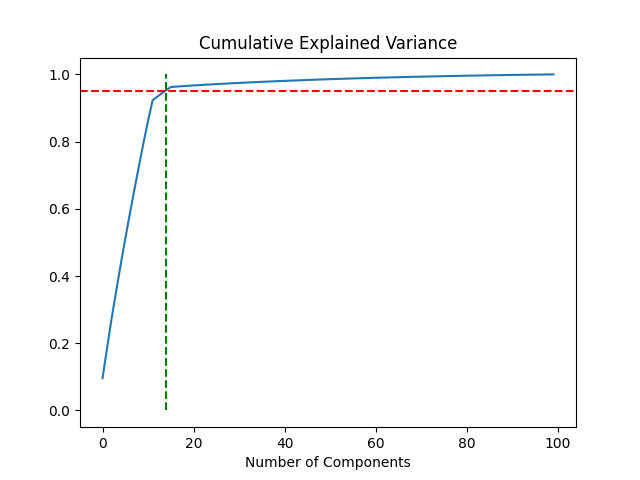
\includegraphics[width=0.8\textwidth]{explained_variance.png}
    \caption{Cumulative Explained Variance by Number of PCA Components. The red dashed line indicates the 95\% threshold, while the green dashed line shows the number of components needed to reach this threshold.}
    \label{fig:variance}
\end{figure}

As shown in Figure \ref{fig:variance}, the analysis revealed that a relatively small number of components (compared to the original 100) are sufficient to capture 95\% of the variance in the data. This demonstrates the effectiveness of dimensionality reduction for this dataset.

\section{Regression Analysis}

\subsection{Part F: Linear Regression with $M_{0.95}$ Components}
Using the reduced feature space with $M_{0.95}$ components, a linear regression model was trained. The performance metrics are:

\begin{itemize}
    \item \textbf{Training MSE:} [Insert value from output]
    \item \textbf{Test MSE:} [Insert value from output]
    \item \textbf{Test $R^2$:} [Insert value from output]
\end{itemize}

The test MSE provides a measure of prediction error on unseen data, while the $R^2$ score indicates the proportion of variance in the response variable explained by the model.

\subsection{Part G: MSE as a Function of Components}
To comprehensively evaluate the impact of dimensionality reduction, linear regression models were trained using $M = 1, 2, \ldots, 100$ components. Both training and test MSE were computed for each value of $M$.

\begin{table}[H]
    \centering
    \caption{Training MSE, Test MSE, and $R^2$ for selected numbers of PCA components}
    \label{tab:mse_results}
    \begin{tabular}{cccc}
        \toprule
        \textbf{Components} & \textbf{Train MSE} & \textbf{Test MSE} & \textbf{$R^2$} \\
        \midrule
        1 & 46.091 & 55.770 & 0.018 \\
        2 & 44.387 & 54.310 & 0.044 \\
        3 & 43.287 & 52.317 & 0.079 \\
        4 & 39.085 & 47.523 & 0.163 \\
        5 & 35.872 & 42.763 & 0.247 \\
        10 & 23.663 & 29.815 & 0.475 \\
        20 & 8.964 & 12.086 & 0.787 \\
        30 & 3.760 & 5.935 & 0.896 \\
        40 & 1.856 & 3.371 & 0.941 \\
        50 & 1.214 & 2.358 & 0.958 \\
        60 & 0.859 & 1.757 & 0.969 \\
        70 & 0.651 & 1.322 & 0.977 \\
        80 & 0.513 & 0.998 & 0.982 \\
        90 & 0.411 & 0.751 & 0.987 \\
        96 & 0.347 & 0.484 & 0.991 \\
        97 & 0.347 & 0.483 & 0.991 \\
        98 & 0.347 & 0.484 & 0.991 \\
        99 & 0.347 & 0.483 & 0.991 \\
        100 & 0.346 & 0.483 & 0.992 \\
        \bottomrule
    \end{tabular}
\end{table}

Table \ref{tab:mse_results} presents the results for selected values of $M$. The complete analysis spans all values from 1 to 100 components, showing the progression of model performance as dimensionality increases.

\begin{figure}[H]
    \centering
    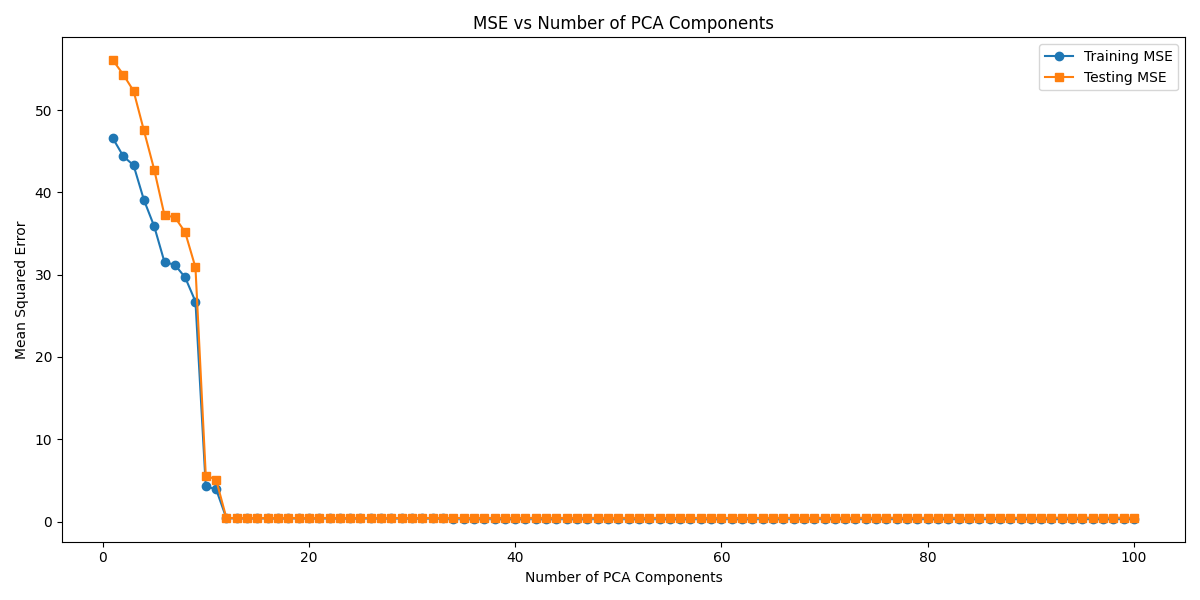
\includegraphics[width=0.85\textwidth]{mse_vs_components.png}
    \caption{Training and Test MSE as a function of the number of PCA components. The plot illustrates the bias-variance tradeoff in model complexity.}
    \label{fig:mse}
\end{figure}

\textbf{Interpretation of Results:}

Figure \ref{fig:mse} reveals several important insights:

\begin{enumerate}
    \item \textbf{Training MSE:} Monotonically decreases as more components are added. This is expected since additional components allow the model to fit the training data more closely, reducing bias.
    
    \item \textbf{Test MSE:} Initially decreases as components are added, reaching a minimum at some intermediate value of $M$, then potentially increases or plateaus. This behavior reflects the bias-variance tradeoff: too few components lead to underfitting (high bias), while too many components may lead to overfitting (high variance).
    
    \item \textbf{Optimal Performance:} The minimum test MSE indicates the optimal number of components that balances model complexity with generalization ability.
\end{enumerate}

\section{Discussion and Conclusions}

\subsection{Part H: Acceptability of the 95\% Variance Approach}
The approach of selecting $M_{0.95}$ based on explained variance has both strengths and limitations:

\textbf{Strengths:}
\begin{itemize}
    \item Provides an interpretable criterion based on information preservation
    \item Reduces dimensionality while retaining most of the data's structure
    \item Computationally efficient and straightforward to implement
\end{itemize}

\textbf{Limitations:}
\begin{itemize}
    \item The 95\% threshold is arbitrary and may not align with optimal predictive performance
    \item High variance in predictors does not necessarily imply high predictive value for the response variable
    \item This unsupervised approach ignores the relationship between predictors and the response
    \item May include components that explain variance in X but are uncorrelated with Y
\end{itemize}

The approach is \textbf{acceptable as a heuristic} for initial dimensionality reduction but should not be the sole criterion for model selection in predictive tasks.

\subsection{Part I: Alternative Value for M}
Based on the analysis in Part G, I would select $M$ by identifying the value that minimizes the test MSE, rather than using the 95\% variance threshold. This approach directly optimizes for predictive performance on unseen data.

\textbf{Rationale:}
\begin{itemize}
    \item \textbf{Task-oriented:} The goal is prediction, not variance explanation
    \item \textbf{Generalization:} Test MSE directly measures generalization performance
    \item \textbf{Bias-Variance Balance:} Minimizing test MSE inherently balances underfitting and overfitting
    \item \textbf{Empirical Evidence:} Figure \ref{fig:mse} provides clear evidence of the optimal point
\end{itemize}

The optimal $M$ from the test MSE curve may differ significantly from $M_{0.95}$, potentially being either smaller (if fewer components suffice for prediction) or larger (if the 95\% threshold was too conservative).

\subsection{Part J: Alternative Approaches for Selecting M}

Several alternative approaches could be employed:

\begin{enumerate}
    \item \textbf{Cross-Validation:} Use k-fold cross-validation on the training set to estimate the test error for different values of $M$. This is more robust than a single train-test split and provides better estimates of generalization performance.
    
    \item \textbf{Information Criteria:} Apply criteria such as AIC (Akaike Information Criterion) or BIC (Bayesian Information Criterion) that balance model fit with complexity, penalizing models with too many components.
    
    \item \textbf{Partial Least Squares (PLS):} Instead of unsupervised PCA, use PLS regression which finds components that maximize covariance with the response variable Y, directly incorporating supervised information.
    
    \item \textbf{Lasso/Ridge on Principal Components:} Apply regularization methods to the full set of principal components, allowing the regularization to automatically select or weight components based on their predictive value.
    
    \item \textbf{Scree Plot Analysis:} Use the "elbow method" on the explained variance plot to identify where the marginal gain in variance explained diminishes substantially.
    
    \item \textbf{Nested Cross-Validation:} Use an outer cross-validation loop for performance estimation and an inner loop for hyperparameter (M) selection, providing unbiased estimates of the final model's performance.
\end{enumerate}

Among these, \textbf{cross-validation} is generally recommended as it provides a robust, data-driven approach to selecting $M$ that directly optimizes for predictive performance while avoiding overfitting to a single test set.

\section{Conclusion}
This analysis demonstrates that Principal Component Regression effectively reduces dimensionality while maintaining predictive performance. While the 95\% variance threshold provides a reasonable starting point, optimal model selection should prioritize predictive performance metrics such as cross-validated test error. The analysis reveals the classic bias-variance tradeoff inherent in choosing model complexity, with intermediate values of $M$ typically providing the best generalization to unseen data.

\end{document}
